%% v3.2 [2019/03/19]
%\documentclass[Proof,technicalreport]{ieicej}
\documentclass[technicalreport]{ieicej-rev}
%\usepackage{graphicx}
\usepackage[dvipdfmx]{graphicx,xcolor}
\usepackage[T1]{fontenc}
\usepackage{lmodern}
\usepackage{textcomp}
\usepackage{latexsym}
\usepackage{url}
\usepackage{cite}
\usepackage{bm}
\usepackage{amsmath}
%\usepackage[fleqn]{amsmath}
%\usepackage{amssymb}
\renewcommand{\figurename}{図}
\renewcommand{\tablename}{表}

\def\IEICEJcls{\texttt{ieicej.cls}}
\def\IEICEJver{3.2}
\newcommand{\AmSLaTeX}{%
 $\mathcal A$\lower.4ex\hbox{$\!\mathcal M\!$}$\mathcal S$-\LaTeX}
%\newcommand{\PS}{{\scshape Post\-Script}}
\def\BibTeX{{\rmfamily B\kern-.05em{\scshape i\kern-.025em b}\kern-.08em
 T\kern-.1667em\lower.7ex\hbox{E}\kern-.125em X}}

\field{D}
\jtitle{IoT端末を考慮したシグナリング制御による\\モバイルコアノードの資源利用の効率化}

\authorlist{
 \authorentry[to-adachi@ist.osaka-u.ac.jp]{安達 智哉}{Tomoya ADACHI}{Osaka}
 \authorentry[s-abe@ist.osaka-u.ac.jp]{阿部 修也}{Shuya ABE}{Osaka}%
 \authorentry[hasegawa@riec.tohoku.ac.jp]{長谷川 剛}{Go HASEGAWA}{Tohoku}%
 \authorentry[murata@ist.osaka-u.ac.jp]{村田 正幸}{Masayuki MURATA}{Osaka}%
}
\affiliate[Osaka]{大阪大学大学院情報科学研究科\hskip1zw
  〒565--0871 大阪府吹田市山田丘1--5}
  {Grad. Sch. of Information Science and Technology,Osaka Univ.,1--5 Yamadaoka,Suita,565--0871,Japan}
\affiliate[Tohoku]{東北大学電気通信研究所\hskip1zw
  〒980--0812 宮城県仙台市青葉区片平二丁目1番1号}
{Research Institute of Electrical Communication,Tohoku Univ.,2--1--1 Katahira,Aoba-ku,Sendai,980--0812,Japan}

% \MailAddress{$\dagger$hanako@denshi.ac.jp,
% $\dagger\dagger$\{taro,jiro\}@jouhou.co.jp}

\renewcommand{\baselinestretch}{0.85}
\begin{document}
\begin{jabstract}
モバイルネットワーク事業者は,自身が運用するモバイルコアネットワークのノード資源が枯渇しないように,収容端末台数や接続頻度に応じて資源割り当てを行う必要がある.一方,近年増加しているIoT端末は,接続される端末の台数を予測することは困難である.また,端末の通信開始時のシグナリング手順を削減するために,RRC Connected Inactive と呼ばれる状態を導入し,端末情報をメモリに一時的に保存することが検討されている.これらのことから,今後,モバイルコアネットワークノードへのCPU負荷やメモリ使用量が大きく変動することが予想され,効率的な資源割り当てが求められる.そこで本報告ではモバイルコアネットワークノードにおけるCPUとメモリ間の負荷のオフロード手法を提案する.具体的には,ネットワークの負荷に合わせて端末の状態を制御することにより,モバイルコアネットワークノードのCPU負荷およびメモリ使用量のバランスを調整し,収容可能な端末台数を最大化する.端末の状態制御は,端末がデータ送受信後にアイドル状態に遷移するまでの時間を制御することで実現する.提案手法により,モバイルコアネットワークノードの資源を増強することなく,収容可能な端末台数が最大で約150\%向上することを示す.
\end{jabstract}
\begin{jkeyword}
モバイルコアネットワーク,IoT通信,資源割り当て,RRC Connected Inactive
\end{jkeyword}
\maketitle




\section{まえがき}
\label{sec:abs}
モバイルネットワーク事業者は,自身が運用するモバイルコアネットワークのノード資源が枯渇しないように,収容端末台数や接続頻度に応じて資源割り当てを行う必要がある.
主なノード資源として,CPUおよびメモリが挙げられる.
CPUは,アタッチやデタッチ等のシグナリングに関する通信や処理を実行するために必要とされる資源である.
一方メモリは,ベアラなどの端末のセッション情報を保持するために必要とされる資源である.
これらのノード資源は,モバイルコアネットワークにおける通信を実現するために必須であり,どちらか一方でも枯渇することは許されない.


一方,近年はIoT端末の急激な増加が注目されている.
IoT端末は,スマートフォンのようなユーザ端末とは異なり,家電や自動車,電気メータ,センサなど様々な場所,様々な用途で使用される可能性があり,端末の台数およびその分布を予測することは困難である.
そのため,多数のIoT端末を収容するためにノード資源を過不足なく割り当てることは難しい.

また,IoT端末はスマートフォン等の従来の端末とはその通信特性が異なり,データ送信に周期性や間欠性を持つという特徴がある.
そのため,データ送信ごとにアイドル状態と接続状態を遷移することが予想される.
その結果,端末のネットワーク接続やデータ送信に必要なシグナリングに関する通信や処理を行う,制御プレーンの輻輳が悪化すると考えられる.
このような問題に対し,RRC Connected Inactiveと呼ばれる新たな状態を導入することによって,特にIoT端末を対象に,シグナリング手順の削減を目標とする研究が行われている\cite{RRCStateHandlingfor5G,ANovelStateModelfor5GRadioAccessNetworks}.
RRC Connected Inactive状態とは,端末がネットワークから切り離された後も,端末のセッション情報をモバイルコアネットワークノードのメモリに保持している状態である.
端末のセッション情報を破棄するアイドル状態とは異なり,モバイルコアネットワークノードのメモリ使用量が増加する一方で,その端末が再び接続状態へ遷移する際に発生するシグナリング手順の一部を省略できるため,CPU負荷の削減が可能となり,制御プレーンの輻輳の抑制が期待できる.
文献\cite{RRCStateHandlingfor5G,ANovelStateModelfor5GRadioAccessNetworks}においては,RRC Connected Inactiveを導入することにより,シグナリングオーバヘッドの削減が可能であることが示されている.


このように,接続台数の予測が難しいIoT端末の普及や,モバイルコアネットワークノードに与える負荷を変化させるような新たな状態の導入により,モバイルコアネットワークノードのCPU負荷やメモリ使用量が時間的に大きく変動することが予想される.
そのため,モバイルネットワーク事業者は,これまで以上に効率的に資源割り当てを行う必要がある.


上述のような資源需要の予測が難しく,変動が激しいモバイルコアネットワークにおいて,収容可能な端末台数の増加を目的とした既存研究として,稼働するサーバやインスタンスの数を需要に応じて増減させる手法が提案されている\cite{Scale-OutArchitectureforServiceOrderProcessingSystems,ACloudNativeSolutionforDynamicAutoScalingofMMEinLTE,OntheScalabilityof5GCoreNetworkTheAMFCase,DynamicAutoScalingAlgorithm(DASA)for5GMobileNetworks,AnAdaptiveScalingMechanismforManagingPerformanceVariationsinNetworkFunctionsVirtualizationACaseStudyinanNFVBasedEPC}.
しかし,そのような手法では,本来必要とされているよりも多くの資源が供給される問題がある.
なぜなら,サーバやインスタンス一台あたりの資源構成は固定であることが一般的であり,偏った資源需要に対してサーバやインスタンスを増加すると,本来増強する必要のない資源も供給されるためである.
文献\cite{ACloudNativeSolutionforDynamicAutoScalingofMMEinLTE}では,IoT端末を収容しているMMEのノード台数を単純に増加すると,一部の資源が過剰に供給される可能性があることを述べている.

また,サーバの資源を効率よく活用するためにサーバの資源を分離し,各資源を個別に増強,更新可能とするServer Disaggregationアーキテクチャが提案されている\cite{TechnoEconomicFrameworkforCloudInfrastructureACostStudyofResourceDisaggregation,IntelsDisaggregatedServerRack,EnhancedBackoffTimerSolutionforGTPCOverloadControl,DisaggregatedandOpticallyInterconnectedMemoryWhenwillitbecosteffective,DisaggregatedServersDriveDataCenterEfficiencyandInnovation,UnderstandingRackScaleDisaggregatedStorage}.
文献\cite{TechnoEconomicFrameworkforCloudInfrastructureACostStudyofResourceDisaggregation}では,Server Disaggregationアーキテクチャをデータセンタに適用することで,CPUやメモリなどの資源を需要に合わせて自由に組み替えることが可能になり,資源の効率的な利用が可能であることが示されている.
しかし,Server Disaggregationは,年単位などの長期的なサーバ更新のためのアーキテクチャであり,本報告で対象とするような突発的な負荷変動に対応することを目的とした方式ではない.
文献\cite{UnderstandingRackScaleDisaggregatedStorage}では,Server Disaggregationアーキテクチャを適用したシステムにおいて,細かい時間粒度で資源制御を行った場合,サーバ資源の再割り当て処理に伴う遅延やコスト面でのオーバーヘッドが大きくなることが示されている.

本報告では,モバイルコアネットワークの端末収容を対象とし,柔軟かつ効率的な,ノード資源の制御手法を提案する.
具体的には,モバイルコアネットワークの負荷に応じて,端末の状態を制御することにより,モバイルコアネットワークノードのCPU負荷およびメモリ使用量を調整することで,収容可能な端末台数を最大化する.
端末の状態の制御は,端末が最後にデータを送信したあと,Connected Inactive状態からアイドル状態に遷移するまでの時間を適応的に設定することで実現する.
さらに,提案手法によるモバイルコアネットワークの性能向上に関する解析的評価を行う.
具体的には,端末の通信状態に応じて発生する,モバイルコアネットワークの負荷を数学的解析によって導出し,我々の研究グループの実験結果などを用いて,定量的な評価を行う.

本報告の構成は以下の通りである.
第\ref{sec:モバイルコアネットワークアーキテクチャ}章では,本報告において評価対象となるモバイルコアネットワークの構成,シグナリング手順および端末の状態遷移について述べる.
第\ref{sec:propose}章では,提案手法について述べる.
第\ref{sec:解析}章では,数学的解析によって,モバイルコアネットワークに発生するCPU負荷およびメモリ使用量を導出する.
第\ref{sec:数値評価}章では,定量的な評価を行うためにパラメータを設定し,提案手法がモバイルコアネットワークの収容可能な端末台数に与える影響を評価する.
最後に第\ref{sec:まとめと今後の課題}章で本報告のまとめと今後の課題について述べる.



\section{モバイルコアネットワークアーキテクチャ}
\label{sec:モバイルコアネットワークアーキテクチャ}
  \subsection{ネットワーク構成}
    図\ref{networkmodel}にモバイルコアネットワークを示す.図中の各ノードは,以下に示す機能を持つ.
    \begin{itemize}
      \item \textbf{User Equipment (UE):} スマートフォンやタブレット,IoTなどの端末.
      \item \textbf{evolved NodeB (eNodeB):} UEと無線で通信を行い,MMEおよびS/PGWとシグナリングメッセージやユーザデータを交換する無線基地局.
      \item \textbf{Mobility Management Entity (MME):} UEやユーザの認証,UEの移動管理およびパケットの経路設定の制御などを行い,モバイルコアネットワークにおけるシグナリングに関する処理の中核となるノード.
      \item \textbf{Serving Gateway / Packet Data Network Gateway (S/PGW):} MMEからのシグナリングメッセージに基づいて,モバイルコアネットワークと外部のネットワーク(External IP Network) を接続するノード.UEがeNodeB間を移動した際のアンカーポイントとしても機能する.
      \item \textbf{Home Subscliber Server (HSS):} ユーザごとの契約情報,認証用のキーデータおよびMMEのアドレスなどの情報を管理するデータベースノード.
    \end{itemize}
    \begin{figure}[!t]
      \centering
      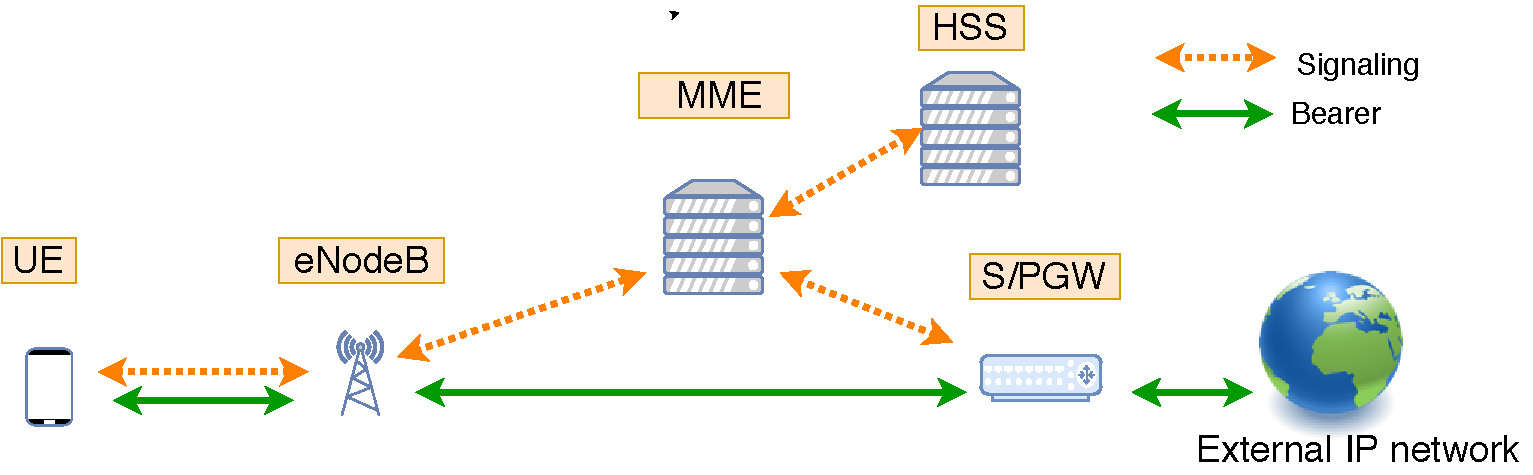
\includegraphics[width=1\hsize]{networkmodel.pdf}
      \caption{モバイルコアネットワークモデル}
      \label{networkmodel}
    \end{figure}

  \subsection{シグナリング手順}
  \label{sec:signaling}
  図\ref{networkmodel}のモバイルコアネットワークにおいて,UEが外部IPネットワークと通信する際,UEとeNodeB間,eNodeBとS/PGW間およびS/PGW内にそれぞれベアラと呼ばれる論理的なトンネルをUE毎に確立する.

  UEは接続状態,アイドル状態,およびConnected Inactive状態という3つの状態を持つものとする.
  接続状態とは,全てのベアラが確立されており,ユーザデータの送受信が可能な状態である.
  アイドル状態とは,ベアラを確立していない状態である.
  この状態では,UEの消費電力は小さいが,ユーザデータの送受信を行うためには,シグナリング手順を行い,接続状態へ遷移する必要がある.
  Connected Inactive状態とは,文献\cite{RRCStateHandlingfor5G,ANovelStateModelfor5GRadioAccessNetworks}などで近年検討されているUEの新しい状態であり,UEとeNodeB間のベアラは解放されているが,eNodeBとS/PGW間およびS/PGW内のベアラは保持している状態である.
  この状態では,UEの消費電力は小さく,かつ,接続状態へ遷移するためのシグナリング手順を一部省略することが可能である.
  一方,UEのセッション情報を保持し続ける必要があり,モバイルコアネットワークノードのメモリ使用量が増加する.


  図\ref{Idle_Connect_Signaling}に,アイドル状態およびConnected Inactive状態から接続状態に遷移するためのシグナリング手順を示す.
  図中のreq.,res.,cmp.,cmd.,msg.,ctxtはそれぞれrequest,response,complete,command,message,contextを意味する.
  また,図中で青色で示されている,5番以降のシグナリング処理およびシグナリングメッセージは,Connected Inactive状態から接続状態に遷移する際には省略される.
  \begin{figure}[!t]
    \centering
    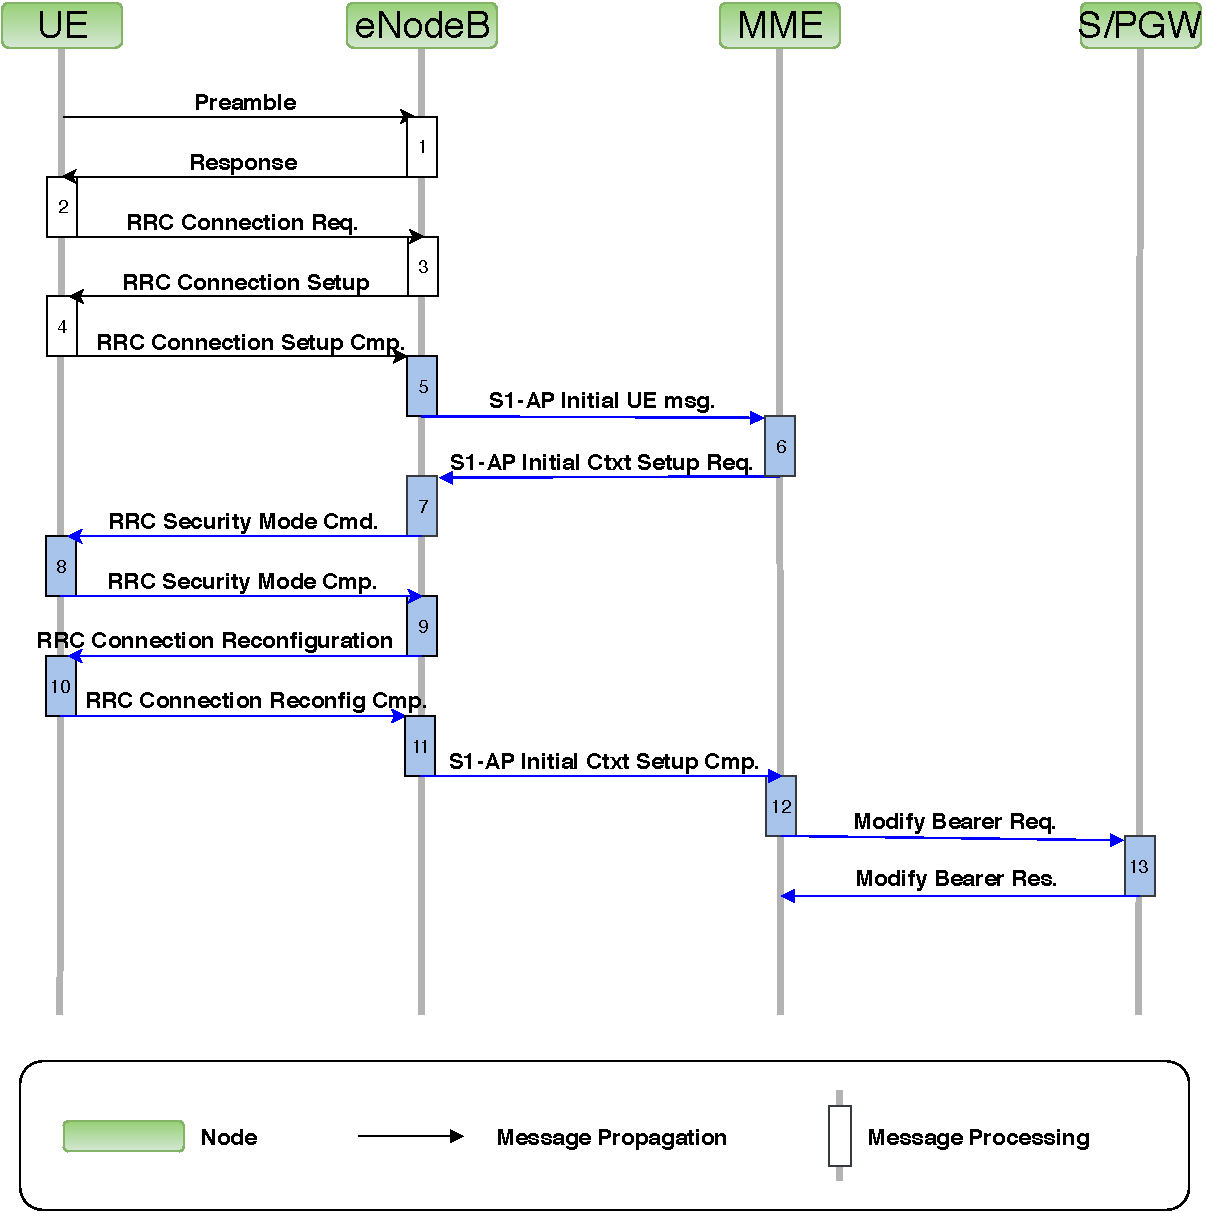
\includegraphics[width=1\hsize]{Idle_Connect_Signaling.pdf}
    % 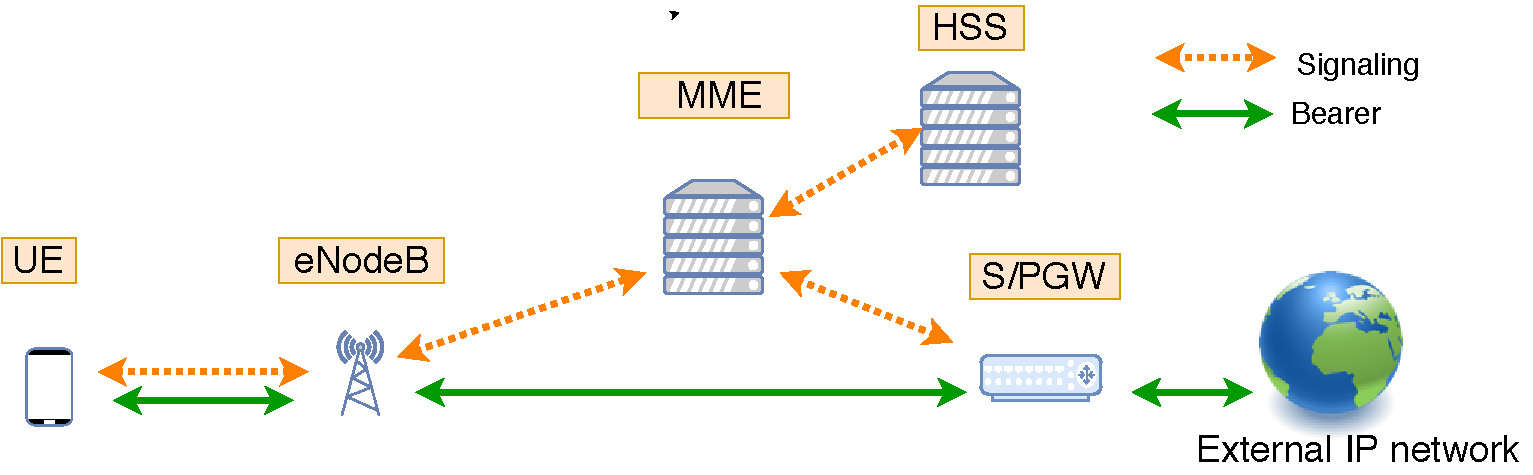
\includegraphics[width=1\hsize]{networkmodel.pdf}
    \caption{アイドル状態およびConnected Inactive状態から接続状態へ遷移する際のシグナリング手順\cite{3gpp.23.720,ANovelStateModelfor5GRadioAccessNetworks}}
    \label{Idle_Connect_Signaling}
  \end{figure}


  \subsection{UEの状態遷移}
  UEの状態遷移図を図\ref{state_change_inactive}に示す.
  図中のConnected,Idle,Connected InactiveはUEの状態を表し,それぞれ接続状態,アイドル状態,Connected Inactive状態に相当する.
  アイドル状態のUEは,データ送信要求が発生すると接続状態へ遷移する.
  その後,Inactiveタイマを起動し,そのタイマが切れるまでデータの送受信が発生しなければ,Connected Inactive状態へ遷移する.
  Connected Inactive状態のUEは,データ送信のタイミングで再び接続状態へ遷移する.
  この時,送信データ量が小さい場合は,接続状態へ遷移することなく,データ送信が行われる.
  これは,シグナリングメッセージに送信データを含めることで実現される.
  \begin{figure}[!t]
    \centering
    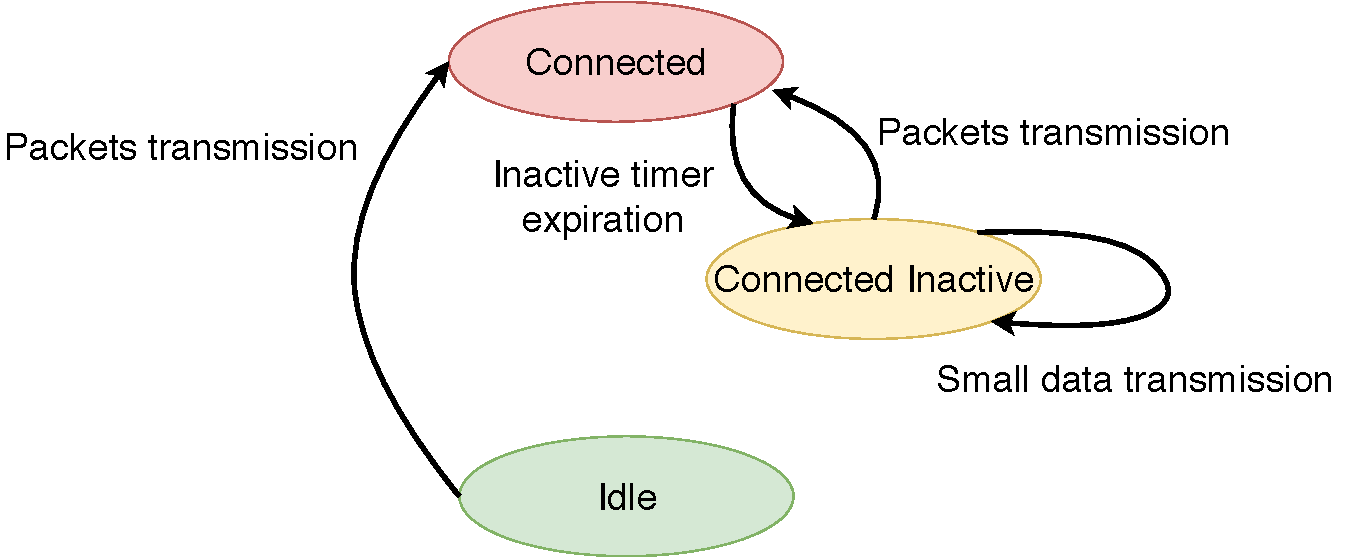
\includegraphics[width=1.0\hsize]{state_change_inactive.pdf}
    \caption{UEの状態遷移図}
    \label{state_change_inactive}
  \end{figure}


\section{提案手法}
\label{sec:propose}
Connected Inactive状態を導入することにより,アイドル状態への遷移が発生しないため,シグナリングメッセージの発生が抑制される.
そのため,モバイルコアネットワークノードのCPU負荷を削減できる.
一方,Connected Inactive状態では,UEのセッション情報を保持するため,モバイルコアネットワークノードのメモリ使用量が増加する.
特に,今後増加すると予想されるIoT端末には通信周期の大きなものがあり,そのようなUEに対してConnected Inactive状態を導入すると,低頻度のデータ送信に対して長期間Connected Inactive状態を維持するため,メモリが浪費される.

この問題に対し,Connected Inactive状態のUEをアイドル状態へ遷移させる新たな状態遷移を導入することで,モバイルコアネットワークノードのCPU負荷およびメモリ使用量を制御することを提案する.
図\ref{state_change_propose}に,提案手法を適用した場合における,UEの状態遷移図を示す.
図\ref{state_change_inactive}と比較して,Connected Inactive状態からアイドル状態への状態遷移が追加されている.
この遷移は,Inactiveタイマとは別の,Idleタイマによって制御される.
UEがデータの送受信を終了したタイミングでIdleタイマが起動し,Idleタイマが切れるまでデータの送受信が発生しなければ,そのUEはアイドル状態へ遷移する.
その際,UEのセッション情報を解放するため,メモリ使用量が削減される.
一方,この遷移はシグナリングを伴うため,モバイルコアネットワークノードのCPU負荷を増加させる.

以上のことから,Idleタイマを適切に設定することによって,モバイルコアネットワークノードのCPU負荷およびメモリ使用量を制御できることがわかる.
提案手法では,Idleタイマを適応的に設定してCPUとメモリ間で負荷をオフロードすることにより,両者の負荷を調整して,モバイルコアネットワークの資源の利用効率を向上する.

\begin{figure}[!t]
  \centering
  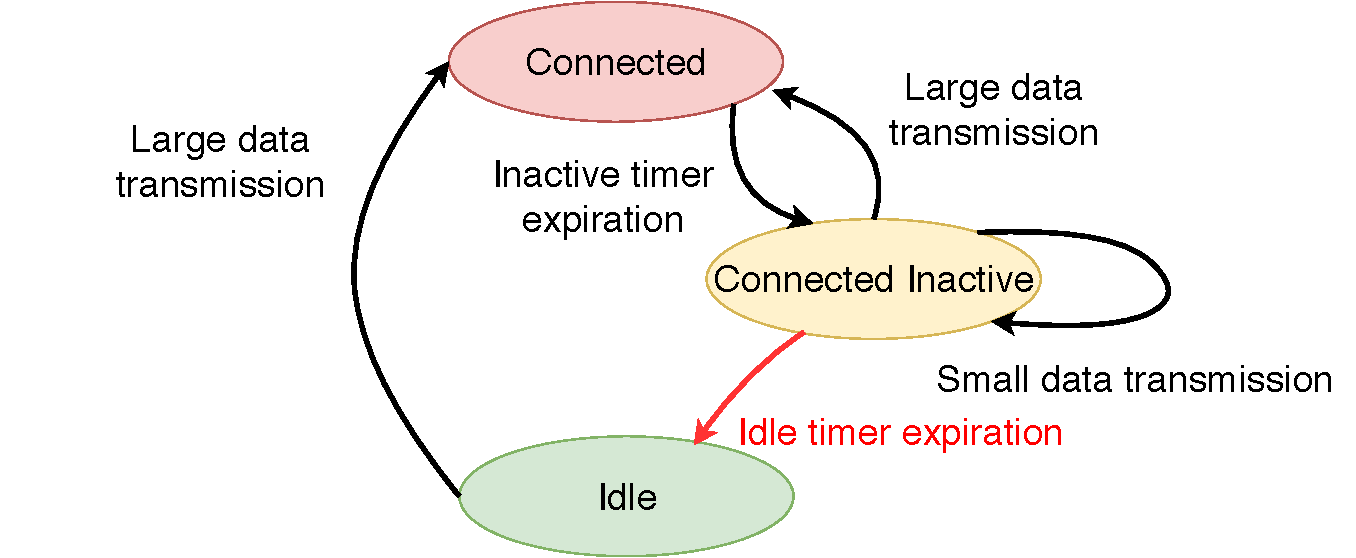
\includegraphics[width=1.0\hsize]{state_change_propose.pdf}
  \caption{提案手法適用したUEの状態遷移図}
  \label{state_change_propose}
\end{figure}


\section{性能解析}
\label{sec:解析}
本章では,提案手法がモバイルコアネットワークの性能に与える影響を定量的に評価することを目的とし,数学的解析に基づくモバイルコアネットワークの負荷の導出を行い,UEの収容可能条件を明らかにする.
% 具体的には,モバイルコアネットワークノードのCPU負荷およびメモリ使用量をそれぞれ第\ref{sec:cpu}節,第\ref{sec:memory}節で導出する.
% また,第\ref{sec:cpu}節および第\ref{sec:memory}節に基づき,収容可能な端末台数を第\ref{sec:syuyo}節で示す.

本章の解析においては,文献\cite{ACloudNativeSolutionforDynamicAutoScalingofMMEinLTE}に基づき,MMEがモバイルコアネットワーク内でのボトルネックになると仮定し,MMEのCPU負荷とメモリ使用量に着目する.
また,対象とするUEは周期的な通信を行い,その周期は既知であると仮定する.
また,一般的にデータプレーンと制御プレーンの資源は分離されていることから,制御プレーンの負荷のみに着目する.
また,データ送信にかかる時間はUEの通信周期と比べて十分小さいものと仮定する.

  \subsection{CPU負荷の導出}
    \label{sec:cpu}
    CPU負荷は1秒あたりにMMEが処理するシグナリングメッセージ数(以下、メッセージ処理頻度と呼ぶ)を基に導出する.
    $N_{\rm UE}$台のUEがモバイルコアネットワークに存在するとし,UEの集合$\bm{U}$を,$\bm{U} = \left\{ u_1,u_2,\ldots,u_{N_{\rm UE}} \right\}$と定義する.
    Inactiveタイマを$T^{\rm ci}$,Idleタイマを$T^{\rm i}$,あるUE $u_h$ $(u_h \in \bm{U})$の通信周期を$T_h$とする.
    % Idleタイマが$T^{\rm i}$であり,UE $u_h$を収容した場合における,MMEのメッセージ処理頻度を$c_h(T^{\rm i})$とする.
    Idleタイマが$T^{\rm i}$である時の,UE $u_h$が1秒あたりに発生させる平均のシグナリングメッセージ数を$c_h(T^{\rm i})$とする.
    また,UEの状態遷移に伴い,MMEに発生するシグナリングメッセージ数をそれぞれ表\ref{table:state}のように定義すると,$c_h(T^{\rm i})$は$T_h$および$T^{\rm ci}$を用いて以下の式(\ref{eq:attach_detach})で表せる.
    ここで,以下では$T^{\rm i} \geq T^{\rm ci}$が常に成り立つものとする.
    \begin{table}[!t]
      \caption{シグナリングメッセージ数の定義}
      \label{table:state}
      \centering
        \begin{tabular}{cc|c}
          \hline
          \multicolumn{2}{c|}{State Transition} & The number of \\
          Source&Destination&signaling messages\\
          \hline \hline
          Connected & Connected & $s_{\rm MME}^{\rm c \to \rm c}$ \\
          Connected Inactive & Connected Inactive & $s_{\rm MME}^{\rm ci \to \rm ci}$ \\
          Connected & Connected Inactive & $s_{\rm MME}^{\rm c \to \rm ci}$ \\
          Connected Inactive & Connected & $s_{\rm MME}^{\rm ci \to \rm c}$ \\
          Connected Inactive & Idle & $s_{\rm MME}^{\rm ci \to \rm i}$ \\
          Idle & Connected  & $s_{\rm MME}^{\rm i \to \rm c}$ \\
          \hline
        \end{tabular}
      \end{table}
    \begin{equation}
      c_h(T^{\rm i})  =
      \begin{cases}
  		    \frac{1}{T_h} \cdot s_{\rm MME}^{\rm c \to \rm c} & \text{if $T_h \le T^{\rm ci}$} \\
          \frac{1}{T_h} \cdot (s_{\rm MME}^{\rm ci \to \rm c} + s_{\rm MME}^{\rm c \to \rm ci}) \cdot d_h  \\\text{     }+ \frac{1}{T_h} \cdot s_{\rm MME}^{\rm ci \to \rm ci} \cdot (1 - d_h) & \text{if $T^{\rm ci} < T_h \le T^{\rm i}$} \\
          \frac{1}{T_h} \cdot (s_{\rm MME}^{\rm i \to \rm c} + s_{\rm MME}^{\rm c \to \rm ci} + s_{\rm MME}^{\rm ci \to \rm i}) & \text{otherwise}
      \end{cases}
      \label{eq:attach_detach}
    \end{equation}
    ここで,$d_h$はUE $u_h$がデータ送信の際に接続状態へ遷移する確率を表す.
    これは,Connected Inactive状態のUEは,送信データ量が閾値より小さいとき,接続状態へ遷移せずにデータ送信を行うことを考慮している.

    MMEのメッセージ処理頻度の平均を$C(T^{\rm i})$と定義する.
    $C(T^{\rm i})$は$c_h(T^{\rm i})$を用いて以下の式(\ref{eq:CPU_load_all_UE})で表せる.
    \begin{eqnarray}
        C(T^{\rm i}) = \sum_{h = 1}^{N_{\rm UE}} c_h(T^{\rm i}) \label{eq:CPU_load_all_UE}
    \end{eqnarray}

  \subsection{メモリ使用量の導出}
    \label{sec:memory}
    Idleタイマが$T^{\rm i}$である時の,UE $u_h$が接続状態である時間割合を$\tau^{\rm c}_h(T^{\rm i})$,Connected Inactive状態である時間割合を$\tau^{\rm ci}_h(T^{\rm i})$,アイドル状態である時間割合を$\tau^{\rm i}_h(T^{\rm i})$と定義する.
    これらは,$T_h$および$T^{\rm ci}$を用いて以下の式(\ref{eq:connected}),(\ref{eq:inactive}),(\ref{eq:idle})で表せる.
    \begin{align}
      \tau^{\rm c}_h(T^{\rm i}) & =
      \begin{cases}
        1 \hphantom{100000000000000} & \text{if $T_h \le T^{\rm ci}$}\\
        \frac{T^{\rm ci}}{T_h} \cdot d_h + \frac{0}{T_h} \cdot (1 - d_h)& \text{if $T^{\rm ci} < T_h \le T^{\rm i}$}\\
        \frac{T^{\rm ci}}{T_h} & \text{otherwise}
      \end{cases} \label{eq:connected}\\
      \tau^{\rm ci}_h(T^{\rm i}) & =
      \begin{cases}
        0 \hphantom{100000000000000} & \text{if $T_h \le T^{\rm ci}$}\\
        \frac{T_h - T^{\rm ci}}{T_h} \cdot d_h + \frac{T_h}{T_h} \cdot (1 - d_h) & \text{if $T^{\rm ci} < T_h \le T^{\rm i}$}\\
        \frac{T^{\rm i} - T^{\rm ci}}{T_h} & \text{otherwise}
      \end{cases} \label{eq:inactive}\\
      \tau^{\rm i}_h(T^{\rm i}) & =
      \begin{cases}
        0 \hphantom{100000000000000} & \text{if $T_h \le T^{\rm ci}$}\\
        0 & \text{if $T^{\rm ci} < T_h \le T^{\rm i}$}\\
        \frac{T_h - T^{\rm i}}{T_h} & \text{otherwise}
      \end{cases}\label{eq:idle}
    \end{align}
    各状態におけるメモリ使用量をそれぞれ表\ref{table:state_memory}のように定義すると,UE $u_h$がMMEに与えるメモリ使用量の平均$m_h(T^{\rm i})$は以下の式(\ref{eq:memory_load})で表せる.
    \begin{table}[!t]
     \caption{MMEのメモリ使用量の定義}
     \label{table:state_memory}
     \centering
      \begin{tabular}{cc}
       \hline
       State & Memory consumption\\
       \hline \hline
       Connected & $m^{\rm c}_{\rm MME}$ \\
       Connected Inactive & $m^{\rm ci}_{\rm MME}$ \\
       Idle & $m^{\rm i}_{\rm MME}$ \\
       \hline
      \end{tabular}
    \end{table}
    \begin{align}
      m_h(T^{\rm i})  =  m^{\rm c}_{\rm MME} \cdot \tau^{\rm c}_h(T^{\rm i}) + m^{\rm ci}_{\rm MME} \cdot \tau^{\rm ci}_h(T^{\rm i}) + m^{\rm i}_{\rm MME} \cdot \tau^{\rm i}_h(T^{\rm i}) \label{eq:memory_load}
    \end{align}
    MMEに対してネットワーク全体で発生する平均的なメモリ使用量を$M(T^{\rm i})$と定義する.$M(T^{\rm i})$は$m_h(T^{\rm i})$を用いて以下の式(\ref{eq:memory_load_all_UE})で表せる.
    \begin{eqnarray}
      M(T^{\rm i})  =  \sum_{h = 1}^{N_{\rm UE}} m_h(T^{\rm i}) \label{eq:memory_load_all_UE}
    \end{eqnarray}
  \subsection{UEの収容可能条件}
  \label{sec:syuyo}
    MMEが1秒あたりに処理できるシグナリングメッセージ数の最大値およびメモリのサイズをそれぞれ$C^{\rm max}$,$M^{\rm max}$とする.
    この時,以下の式(\ref{eq:all_UE_capacity})に示した2つの条件を同時に満たすような$T^{\rm i}$が存在するならば,与えられたUEは全て収容可能である.
    \begin{eqnarray}
    \begin{split}
      C(T^{\rm i}) &\le C^{\rm max}
      \\ M(T^{\rm i}) &\le M^{\rm max}
      \label{eq:all_UE_capacity}
    \end{split}
    \end{eqnarray}

\section{数値評価}
\label{sec:数値評価}
\subsection{パラメータ設定}
\label{sec:パラメータ設定}
数値評価において用いるパラメータ設定を表\ref{table:parameter}に示す.
Inactive タイマは,文献\cite{ANovelStateModelfor5GRadioAccessNetworks}を参考に,10~sに設定した.
UEの状態遷移に伴うシグナリングメッセージ数は,文献\cite{3gpp.23.720}および\cite{ANovelStateModelfor5GRadioAccessNetworks}に基づき設定した.
文献\cite{3gpp.23.720}および\cite{ANovelStateModelfor5GRadioAccessNetworks}に明示されていない一部の状態遷移に関しては,同様の状態遷移に基づいて決定した.UEの状態に応じたMMEのメモリ使用量は,モバイルコアネットワーク機能を実装したオープンソースソフトウェアであるOpenAirInterface (OAI) \cite{OpenAirInterface}のソースコードに基づき設定した.
具体的には,MMEが保持する情報およびそのサイズを,OAIのソースコードを静的解析することにより導出し,メモリ使用量を決定した.
Connected Inactive状態はOAIで実装されていなため,文献\cite{3gpp.23.720}および\cite{ANovelStateModelfor5GRadioAccessNetworks}に基づくシグナリング手順を踏まえ,接続状態と同等のメモリ使用量と推定した.
MMEが1秒あたりに処理できるシグナリングメッセージ数は文献\cite{ExperimentalEvaluationofMobileCoreNetworksonSimultaneousAccessfromM2MIoTTerminals}を基に設定した.文献\cite{ExperimentalEvaluationofMobileCoreNetworksonSimultaneousAccessfromM2MIoTTerminals}では,OAIを用い,アタッチ要求の頻度とMMEの処理時間との関係を実験により評価し,短時間に多数のアタッチ要求をMMEが受け付けた場合,MMEの処理遅延時間が急激に増加することを示している.本報告では,文献\cite{ExperimentalEvaluationofMobileCoreNetworksonSimultaneousAccessfromM2MIoTTerminals}においてMMEの処理遅延時間が急激に増加するメッセージ処理頻度に基づき,MMEが1秒あたりに処理できるシグナリングメッセージ数を1,200とした.また,MMEのメモリサイズは1,000~MBとした.また,UEの送信データサイズは十分大きいものとし,データ送信の際は必ず接続状態に遷移すると考え,$d_h = 1$とした.
\begin{table}[!t]
  \centering
  \caption{パラメータ設定}
  \label{table:parameter}
  \begin{tabular}{c|l}
    \hline
    Parameter  & Numerical setting \\\hline \hline
    $T^{\rm ci}$ & 10~s\\
    $s_{\rm MME}^{\rm c \to \rm c}$ & 0~messages\\
    $s_{\rm MME}^{\rm ci \to \rm ci}$ & 0~messages\\
    $s_{\rm MME}^{\rm c \to \rm ci}$ & 0~messages\\
    $s_{\rm MME}^{\rm ci \to \rm c}$ & 0~messages\\
    $s_{\rm MME}^{\rm ci \to \rm i}$ & 5~messages\\
    $s_{\rm MME}^{\rm i \to \rm c}$ & 5~messages\\
    $m^{\rm c}_{\rm MME}$ & 17878~bits\\
    $m^{\rm ci}_{\rm MME}$ & 17878~bits\\
    $m^{\rm i}_{\rm MME}$ & 408~bits\\
    $C^{\rm max}$ & 1200~messages/s\\
    $M^{\rm max}$ & 1,000~MB\\
    $d_h$ & 1 \\\hline
  \end{tabular}
\end{table}

\subsection{評価シナリオ}
\label{sec:estimate4}
本報告では,UEの通信周期が異なる2つのシナリオに対して提案手法を適用した際の性能評価を行う.
シナリオ1では,UE台数が500,000台であり,UEごとの通信周期は10~sから6,000~sの範囲で一様分布とする.
このシナリオでは,一般的にUEの通信周期は明らかでないことを考慮して,UEの通信周期は一様分布であるという簡単な仮定をおいた場合の評価を行う.
シナリオ2では,UE台数が500,000台であり,UEごとの通信周期は文献\cite{3gpp.45.820}に基づき設定した.
具体的には,UEの持つ通信周期は1~day,2~hours,1~hour,30~minutesのいずれかであり,それぞれの通信周期を持つUEの割合は表\ref{table:interval}の通りである.
このシナリオでは,現実的なアプリケーションを想定した評価を行う.
\begin{table}[!t]
  \centering
  \caption{シナリオ2におけるUEの通信周期の分布}
  \label{table:interval}
  \begin{tabular}{c|cccc}
    \hline
    &\multicolumn{4}{c}{通信周期} \\
    & 1~day & 2~hours & 1~hour & 30~minutes \\\hline \hline
    UE台数の割合 & 40\% & 40\% & 15\% & 5\% \\\hline
  \end{tabular}
\end{table}

また,シナリオ2においては,UE台数を変化させた場合の評価も行う.

\subsection{評価結果と考察}
シナリオ1において,Idleタイマを10~sから6,000~sまで変化させた場合における,メッセージ処理頻度とメモリ使用量の関係を図\ref{theory_1_all_30s_theory}に示す.
横軸がメッセージ処理頻度,縦軸がメモリ使用量である.
図中の縦の破線および横の破線はそれぞれ,$C^{\rm max}$および$M^{\rm max}$を表す.
また,グラフの点の色はIdleタイマの値に対応している.
\begin{figure}[!t]
  \centering
  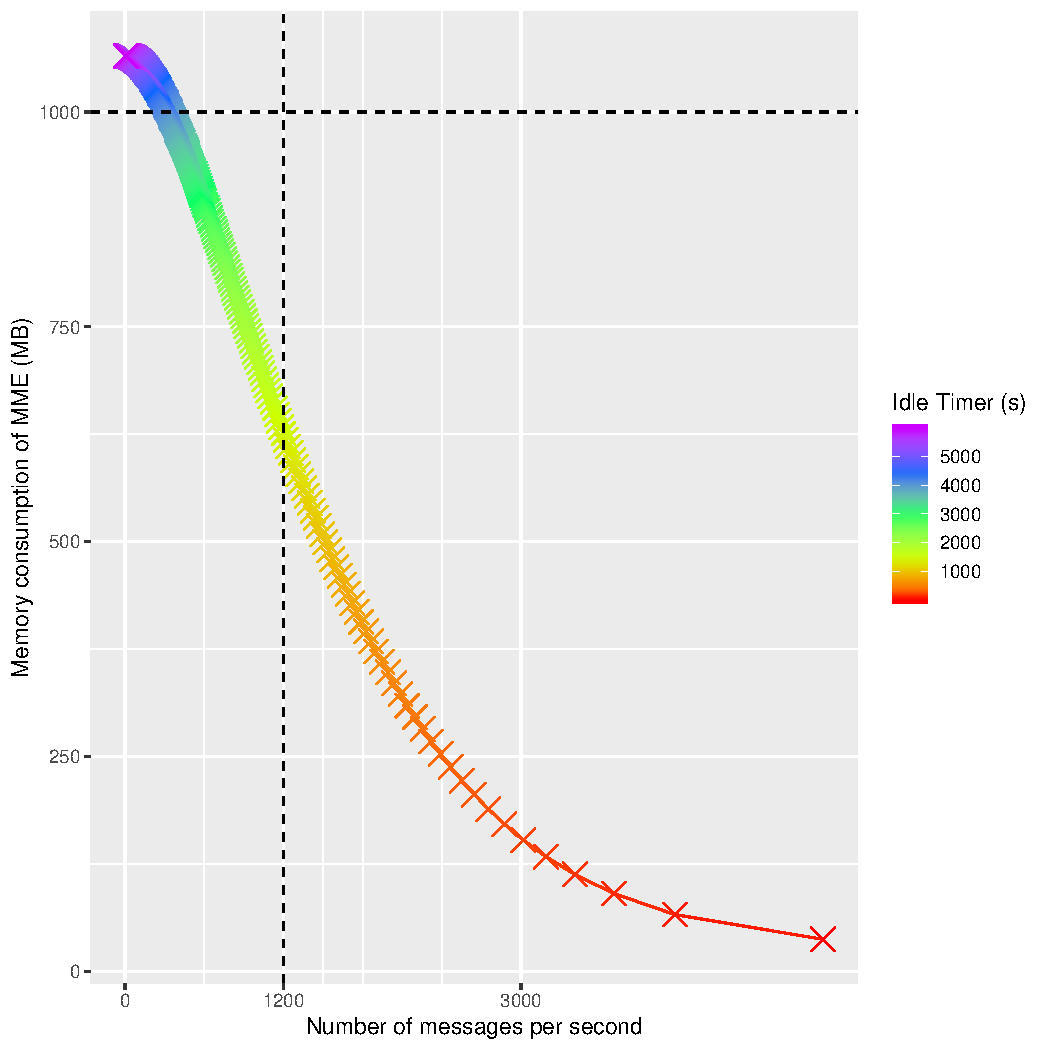
\includegraphics[width=1\hsize]{theory_1_all_30s_theory.pdf}
  \caption{Idleタイマに対する,メッセージ処理頻度とメモリ使用量の関係(シナリオ1)}
  \label{theory_1_all_30s_theory}
\end{figure}
図\ref{theory_1_all_30s_theory}より,Idleタイマの変化に応じて,メッセージ処理頻度およびメモリ使用量が変化することがわかる.
具体的には,Idleタイマが増加すると,メッセージ処理頻度は減少し,メモリ使用量は増加する.
これはIdleタイマの増加に伴い,データ送信後にアイドル状態へと遷移するUEが減少し,シグナリングメッセージが削減される一方,Connected Inactive状態を維持するUEが増加し,MMEが保持する情報が増加するためである.
以上より,Idleタイマの適応的な設定により,CPU負荷とメモリ使用量を互いにオフロードできることが確認できる.
また,Idleタイマが1,422~sより小さい時は,メッセージ処理頻度が$C^{\rm max}$を超え,Idleタイマが4,000~sより大きい時は,メモリ使用量が$M^{\rm max}$を超える.
そのため,本シナリオにおいて全UEを収容するためには,Idleタイマを1,422~s以上,4,000~s以下に設定する必要がある.

シナリオ2において,Idleタイマを10~sから864,000~sまで変化させた場合における,メッセージ処理頻度とメモリ使用量の関係を図\ref{theory_2_all_300s_theory}に示す.
\begin{figure}[!t]
  \centering
  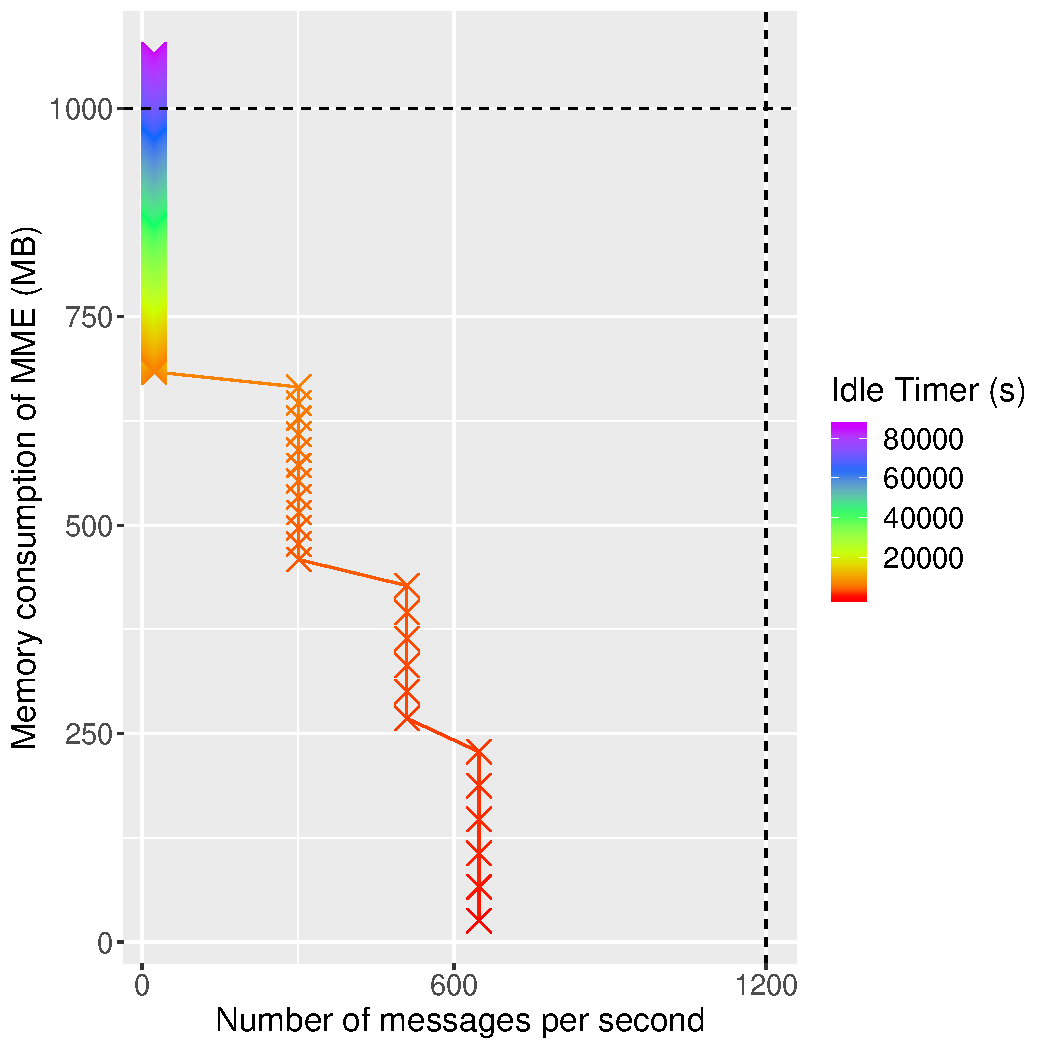
\includegraphics[width=1\hsize]{theory_2_all_300s_theory.pdf}
  \caption{Idleタイマに対する,メッセージ処理頻度とメモリ使用量の関係(シナリオ2)}
  \label{theory_2_all_300s_theory}
\end{figure}
シナリオ1と同様にIdleタイマが大きくなるとメモリ使用量は増加している.
一方,メッセージ処理頻度は段階的に減少している.
これは表\ref{table:interval}に示すようにUEの通信周期の分布が離散的であるためである.
また,Idleタイマが72,789~sより大きい時は,メモリ使用量が$M^{\rm max}$を超える.
そのため,本シナリオにおいて全UEを収容するためには,Idleタイマを72,789~s以下に設定する必要がある.

シナリオ1とシナリオ2を比較すると,UE台数が同じであっても,UEの通信周期の分布が異なると,MMEに発生する負荷が異なり,全てのUEを収容するためのIdleタイマの設定条件が異なることが確認できる.
これは,IoT端末のように通信周期の予測が難しい端末を収容する際には,適応的なIdleタイマの設定を行うことによって,MMEの資源制御を行う必要があることを示している.

最後に,Idleタイマの設定値が収容可能なUE台数に与える影響を評価する.
UEの持つ通信周期およびそのUEの割合はシナリオ2と同じとする.
その上で,UE台数を469,200台,925,700台,および1,178,100台と変化させた時の評価結果を図\ref{10_11_12_signaling_vs_memoryload}に示す.
\begin{figure}[!t]
  \centering
  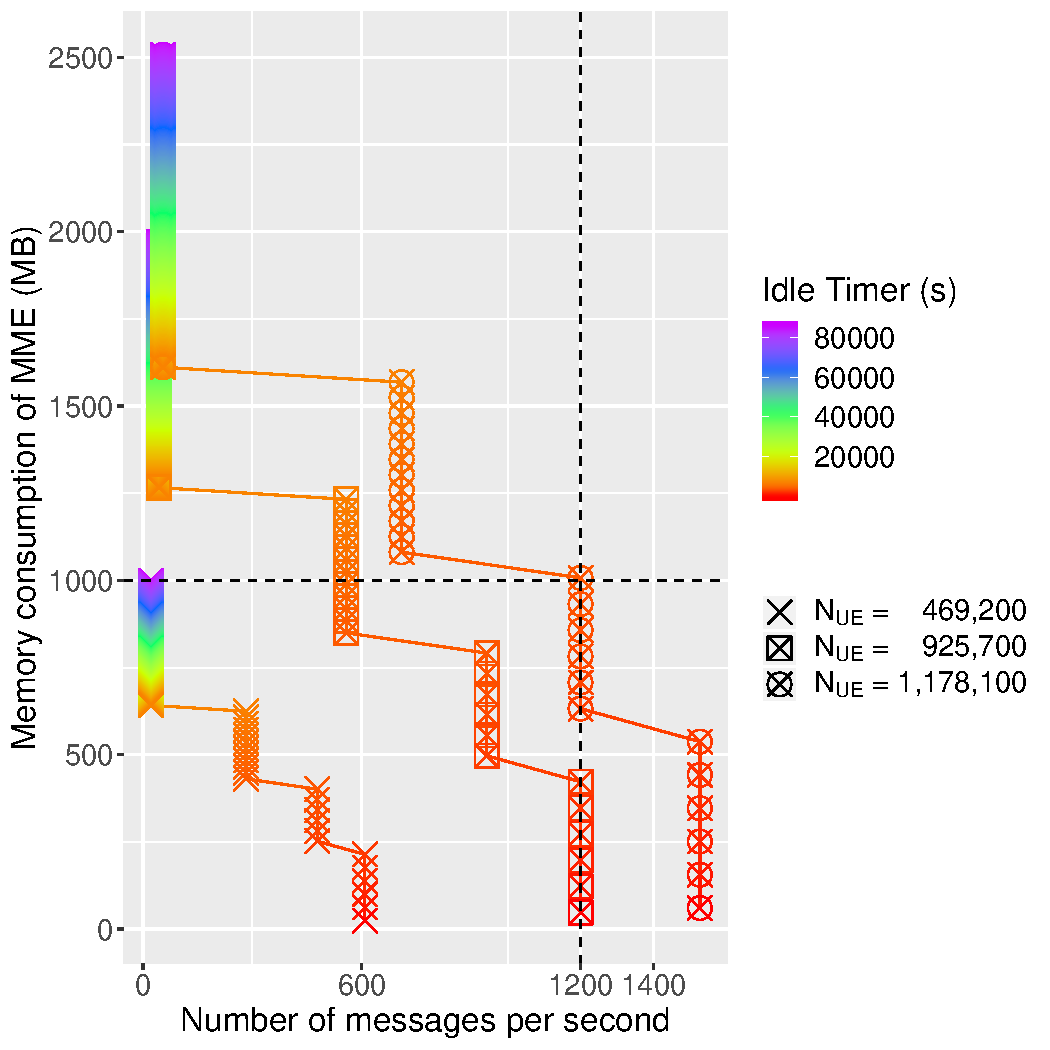
\includegraphics[width=1\hsize]{10_11_12_signaling_vs_memoryload_all_300s_theory.pdf}
  \caption{Idleタイマに対する,メッセージ処理頻度とメモリ使用量の関係(シナリオ2,$N_{\rm UE} = 469,200,925,700,1,178,100$)}
  \label{10_11_12_signaling_vs_memoryload}
\end{figure}
UE台数が469,200台のグラフを見ると,Idleタイマが小さい場合はメッセージ処理頻度およびメモリ使用量は共にシステム容量($C^{\rm max}$,$M^{\rm max}$)を下回っているが,Idleタイマが80,000~s以上の場合,メモリ使用量が$M^{\rm max}$に達している.
これは,Idleタイマに80,000~s以上の値を設定する場合には,収容可能なUE台数が469,200台であることを意味する.
UE台数が925,700台のグラフを見ると,Idleタイマが1,800~s未満の場合,メッセージ処理頻度が$C^{\rm max}$に達している.
これは,Idleタイマに1,800~s未満の値を設定する場合には,収容可能なUE台数が925,700台であることを意味する.
さらに,UE台数が1,178,100台のグラフを見ると,Idleタイマが1,800~s以上3,281~s以下の時,メッセージ処理頻度およびメモリ使用量が$C^{\rm max}$および
$M^{\rm max}$にそれぞれ達している.
これは,Idleタイマを1,800~s以上3,281~s以下に設定する場合には,収容可能なUE台数が1,178,100台であることを意味する.

以上の評価より,Idleタイマの値によって収容可能なUE台数が大きく変化することがわかる.
具体的には,シナリオ2においては,Idleタイマを適切に設定することにより,Idleタイマを80,000~s以上に設定した場合および1,800~s未満に設定した場合と比較して,収容可能なUE台数がそれぞれ151\%および27\%向上する.

提案手法を用いない場合においては,Connected Inactive状態からアイドル状態へ状態遷移が発生しない.
これは,Idleタイマを無限大に設定した場合と透過であり,上述の結果より,収容可能なUE台数は469,200台である.
したがって,シナリオ2においては,提案手法を用いてIdleタイマを適切に設定することにより,提案手法を用いない場合と比較して,収容可能なUE台数が151\%向上するといえる.

\section{まとめと今後の課題}
\label{sec:まとめと今後の課題}
本報告では,モバイルコアネットワークノードの資源利用の効率化を目的とし,端末の状態遷移に関するパラメータ制御による,CPUおよびメモリ間の負荷のオフロード手法を提案した.
具体的には,端末がConnected Inactive状態からアイドル状態へ遷移することを提案し,遷移の条件となるIdleタイマの値を調整することにより,MMEに発生するCPU負荷およびメモリ消費量を制御する。
次に提案手法の評価を行うために,数学的解析に基づいてCPU負荷およびメモリ使用量を導出した.
最後に,端末台数や通信周期が異なるいくつかのシナリオにおいて提案手法を適用した場合の評価を行い,提案手法がCPU負荷およびメモリ使用量に与える影響を明らかにした.
その結果,提案手法を用いることにより,CPU負荷とメモリ使用量を互いにオフロードすることができ,資源利用が効率化されることを確認した.
さらに,特定のシナリオにおいては,提案手法を用いることにより,収容可能な端末台数が最大151\%向上することを確認した.

今後の課題として,Idleタイマの動的かつ適応的な制御手法の検討が挙げられる.
本報告においては,端末台数および通信周期が明らかかつ不変であり,適切なIdleタイマの値が導出できるという前提の下で提案手法の評価を行った.
しかし,一般的に,端末台数および通信周期は未知であり時間的に変動する.
そのような状況においても,Idleタイマを適切に制御できる手法を検討することにより,より現実的なシナリオにおける評価が可能になる.
また,Server Disaggregationアーキテクチャやスケールアウト/スケールイン等と提案手法を組み合わせて,より効率的な資源制御を行うことも検討したい.

\bibliographystyle{IEEEtran}
\bibliography{/Users/t-adachi/Documents/study/Bibliography/bib/hpt_core_network/myBib/LABbiblio,/Users/t-adachi/Documents/study/Bibliography/bib/hpt_core_network/Study_Group_Bibtex/bib/hptCoreNetwork_Study}
\end{document}
